%
% Apéndice sobre servidor de despliegue.
% Reporte técnico.
% Proyecto Lovelace.
%
% TODO:
%  Agrega términos al glosario: máquina virtual, balanceador de carga,
%  software libre.
%

\capitulo[SER]{Sobre el servidor de despliegue}{sec:sobre_el_servidor}{%
  \epigrafe{%
    One reason you should not use web applications to do your computing is that
    you lose control. It's just as bad as using a proprietary program. Do your
    own computing on your own computer with your copy of a freedom-respecting
    program. If you use a proprietary program or somebody else's web server,
    you're defenceless.}{Richard Stallman}}%
%
Este apéndice trata los temas y configuraciones más importantes sobre el
la computadora servidor que, durante el desarrollo de este proyecto, fungió
como entorno de producción. En cada una de las siguientes secciones se tratan
los aspectos más interesantes de las configuraciones y se enlistan las
dependencias más importantes.

\section{Sobre el servicio de \textit{hosting}}

El servidor de desplieque es un \textit{Droplet} de \textit{Digital
Ocean}\footnotemark[1]{}. Los \textit{Droplets} son máquinas virtuales con
sistemas operativos \gls{gl:gnu}/Linux que funcionan como
servidores~\cite{digital_ocean_droplets}. Al crear un \textit{Droplet} es
necesario seleccionar el sistema operativo que tendrá; para el servidor de
desplieugue de este proyecto se ocupa \textit{Debian}:
\hipervinculo{dep:servidor}. Para poder pagar este servicio se
hace uso del programa de \textit{GitHub} de apoyo a
estudiantes\footnotemark[2]{}.

\footnotetext[1]{%
  Empresa dedicada a la renta de recursos de cómputo en línea: máquinas
  virtuales, medios de almacenamiento, balanceadores de carga, entro otros.
  \url{https://www.digitalocean.com/}.}

\footnotetext[2]{%
  Consiste en una serie de promociones para usar algunas herramientas
  relacionadas con el desarrollo de software.
  \url{https://education.github.com/pack}}

\dependencia[dep:servidor]{Sistema operativo}{Debian 9 Stretch}{%
  \acrshort{gl:dfsg}}{https://www.debian.org/}{%
    Sistema operativo \gls{gl:gnu}/Linux. A diferencia de otras
    distribuciones, esta se compone enteramente se software libre.}

El \textit{Droplet} contratado se encuentra en un centro de datos de San
Francisco: de todos los centros disponibles, el más cercano a México; con
la dirección \gls{gl:ip}v4 \texttt{159.65.96.59}. En la
figura~\ref{fig:digital_ocean} se muestra la interfaz de control.

\begin{figure}
  \begin{center}
    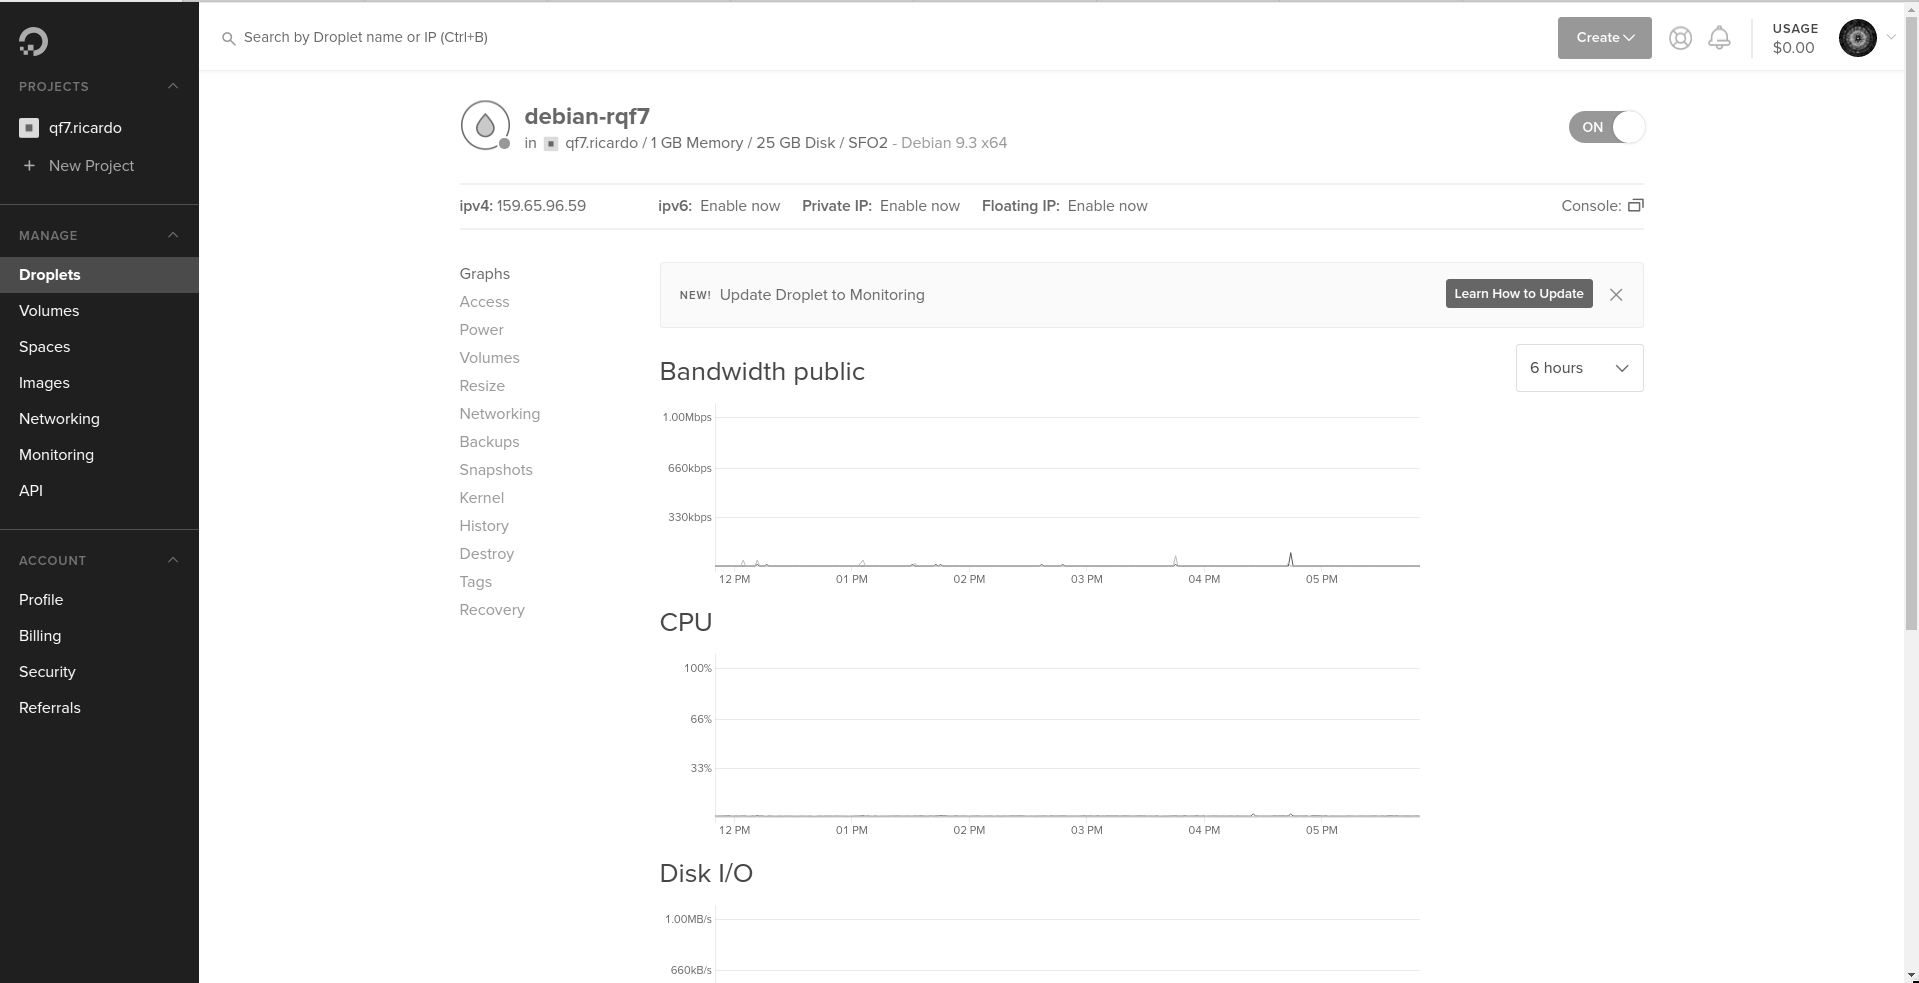
\includegraphics[width=0.75\textwidth]{diagramas/digital_ocean.png}
    \caption{Interfaz de control de \textit{Droplet}.}
    \label{fig:digital_ocean}
  \end{center}
\end{figure}

\section{Sobre el servidor web}

\section{Sobre el servidor de correos electrónicos}

\section{Sobre los certificados \texorpdfstring{%
  \acrshort{gl:ssl}/\acrshort{gl:tls}}{SSL/TLS}}

\section{Sobre el servidor de etiquetas}
